\chapter{SDN中流量测量sketch的研究现状}\label{chap:sketch}

本章将介绍4种典型的用于流量测量的sketch,并分析它们为何无法适用于SDN。

\section{Count-Min\cite{cormode2004improved}}

\begin{figure}[h]
	\centering
	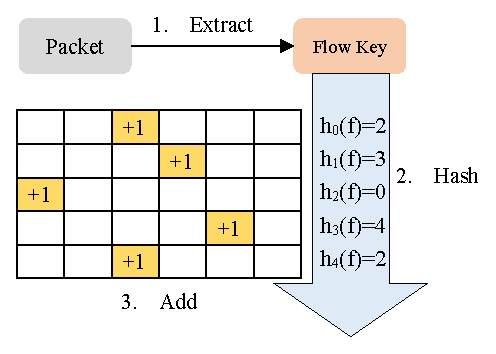
\includegraphics[width=0.8\linewidth]{fig/countmin2.eps}
	\caption{Count-Min的更新过程}\label{fig:countmin}
\end{figure}

如图\ref{fig:countmin}所示,Count-Min sketch的存储形式是一个高度为$d$、长度为$w$的二维数组(也称为\textit{bitmap})。数组中的每个位置称为一个“格子”(slot),格子中包含了一个从0开始的计数器。
数组中的每一行都拥有一个哈希函数,可以将任意流ID,如5元组,映射到$\{0,1,...,w-1\}$之间的某个整数。

当一个数据包到达时,Count-Min首先读取它的流ID,然后对于数组的每一行,使用它的哈希函数将ID映射为一个数,用这个数作为索引定位到相应的格子,将格子中的计数器增加对应的数据包大小。
由哈希函数的特性可知,同一条流的数据包将会一直映射到同样的$d$个格子。

要从Count-Min当中查询某个流的大小,先重复之前的步骤,利用哈希函数定位到具体的格子。因为Count-Min总共有$d$行,所以会找到$d$个格子。选择这些格子当中最小的计数器作为流的大小的估计。
由于哈希碰撞的存在,因此Count-Min的查询结果总是大于或等于实际的大小。

\section{CountSketch \cite{charikar2004finding}}\label{sec:countsketch}
CountSketch \cite{charikar2004finding}和Count-Min有一点相似,它同样拥有一个高度为$d$、长度为$w$的bitmap,以及$d$个将流ID映射成$\{0,1,...,w-1\}$中的整数的哈希函数。
除此之外,CountSketch还另有$d$个将流ID映射成$1$或$-1$的一系列哈希函数。

进行更新操作时,CountSketch首先使用第一套哈希函数来确定格子,再使用第二套哈希函数得到一个$1$或$-1$的系数。将数据包的大小乘上这个系数之后,再加到格子里的计数器上。
也就是说,Count-Min中的计数器只会增加,而CountSketch中的计数器有可能加也有可能减,取决于第二个哈希函数和流的ID。

在bitmap中查询流的大小的过程和Count-Min类似,但和Count-Min不同的是,CountSketch选择的不是$d$个计数值中的最小值,而是中位数。

\begin{figure}
   \centering
   \includegraphics[width=\linewidth]{fig/countsketch.eps}
   \caption{CountSketch的结构}
   \label{fig:countsketch}
\end{figure}

此外,CountSketch还拥有找出top-$k$的流的能力。如图\ref{fig:countsketch}所示,为了记录top-$k$的流,CountSketch维护了一个容积为$k$的小根堆,其中存放了这些大流的ID以及它们的流量。

当数据包抵达时,CountSketch首先更新它的bitmap,然后再检查这个数据包所属的流是否已在堆中。
如果已在堆中,那么就将堆中对应的项目的流量值增加这个数据包的大小;
否则,CountSketch就会在bitmap中执行查询操作,获取当前流的流量估计值。
如果估计值比小根堆中最小的值要大的话,就将这个最小值移出堆,并将当前流的ID和流量估计值加入堆中。或者如果堆还没有满,也会当前流的信息放入堆中。

由于CountSketch的更新过程涉及堆的操作,因而它的计算负载也受堆操作的影响。如果使用简单的小根堆实现,那么更新堆中项目的时间复杂度是$O(\log{k})$, 在堆中查找某条流的时间复杂度是$O(k)$。
对每个数据包,CountSketch都要在堆中进行查找操作,这一过程大幅增大了CountSketch的计算负载。



\section{Filtered Space-Saving \cite{homem2010finding}}\label{sec:FSS}
在严格意义上,Filtered Space-Saving (FSS) \cite{homem2010finding}不能算做一种sketch,而应看做是一种基于“Counter”的算法。然而就实际应用而言这点可以忽略。

FSS由一个只有1行的bitmap和一个容量为$k$的哈希表组成,其中bitmap用于粗略估算流的大小,哈希表则用来精确统计一部分的流的大小。
bitmap中的每个格子包括“计数器”和“指示器”两个字段。计数器用来记录流量统计,指示器则记录了通过哈希函数映射到这个格子中的流当中,有多少条也在哈希表当中。

每当新的数据包抵达,FSS首先用哈希函数将流的ID映射到bitmap中的一个格子,并检查这个格子中的指示器。
如果指示器的数字不为0,FSS会在哈希表中搜索该流ID。若流ID存在于哈希表中,那么哈希表中对应的计数器就增加数据包的大小。
如果指示器是0,或者ID不存在在哈希表中,那么就将bitmap中对应的格子里的计数器增加数据包的大小。
在此之后,若格子中的计数器大于哈希表中的最小值,就将该流的ID和计数器的数字插入哈希表中,并将格子中的指示器加1。
如果在插入时哈希表已满,那么哈希表中数值最小的一条流会被移除。在移除之后,FSS将会利用哈希函数为这条流找到它所对应的格子,将它原本在哈希表中的计数器数字复制到格子中的计数器中,并将格子里的指示器减1。

对于流ID存在于哈希表中的情况,FSS执行更新操作的时间复杂度是$O(1)$。其他情况下,FSS需要寻找哈希表中的最小项,因此时间复杂度是$O(k)$。

\begin{table}[h]
	\centering
	\begin{tabular}{c|c}
		\hline
		Kick-out 频率 & CPU周期/数据包 \\
		\hline
		0.1\% & 59 \\
		\hline
		0.5\% & 108 \\
		\hline
		1\% & 170 \\
		\hline
		2\% & 293 \\
		\hline
		5\% & 661 \\
		\hline
	\end{tabular}
	\caption{SketchVisor的计算负载随kick-out频率的变化}\label{tbl:sketchvisor}
\end{table}

\section{SketchVisor \cite{huang2017sketchvisor}}\label{subsec:sketchvisor}

SketchVisor \cite{huang2017sketchvisor}论文为其中的“Fast Path”设计了一个可以实现top-$k$流统计的算法。此算法维护一个有$k$行的表,表中的每一行包含一个流的ID和3个统计字段。
每到达一个数据包,如果该数据包的流存在于表中,或者表尚未存满,则只是简单的在表中插入或增加对应的表项。否则,整张表内的所有数据都要更新,这种操作被称为“kick-out”。
\cite{huang2017sketchvisor}中的测试结果显示,一个kick-out操作需要12332个CPU时钟周期,普通的更新则只需要47个时钟周期。

根据这一测试结果,我们估算了不同的kick-out比率下处理每个数据包消耗的平均时钟周期数。
如表\ref{tbl:sketchvisor}所示,SketchVisor的计算负载只在kick-out比率不超过1\%时才能够接受。也就是说,SketchVisor的表中所存储的流的流量之和要超过全部流量的99\%。
在实际网络中,由于流是在变化的,用一张表追踪99\%的流量明显不切实际。更何况要囊括更多的流,$k$也要随之增大,导致占用的内存空间也会增大。

\section{现有方法的不足}\label{sec:observation}

\begin{table*}[t]
	\centering
	\begin{tabular}{c|c|c|c|c}
		\hline
		Sketch & 计算负载 &估计误差&大流监测率& 能否识别大流 \\
		\hline
		Count-Min\cite{cormode2004improved} & 低 &低& 无 &否\\
		\hline
		CountSketch\cite{charikar2004finding} & 高 &高 &低&是\\
		\hline
		Filtered Space-Saving\cite{homem2010finding}  & 一般 & 一般&高& 是\\
		\hline
		\textbf{Our Sketch} & 低 &低 &高&是\\
		\hline		
	\end{tabular}
	\caption{不同sketch之间的对比}\label{tbl:sketchcompare}
\end{table*}

前文介绍了Count-Min等4种sketch,接下来对这些sketch的优势和不足进行分析。
Count-Min的主要优势在于它的计算负载极低,并且估计误差较低。但是Count-Min并不记录任何流本身的信息,因而无法筛选出大流。一些研究对Count-Min进行了拓展,使其能够反查大流的信息。
如Deltoid \cite{cormode2005s}使用了额外的计数器来编码流的ID;
Reversible Sketch \cite{schweller2007reversible}将流ID拆分成多个部分并分别进行哈希;
FlowRadar \cite{li2016flowradar}使用连续的异或运算来编码和恢复流的ID。
然而,根据SketchVisor \cite{huang2017sketchvisor}中的测试结果,这些改进算法的计算负载都比较高。

SketchVisor有着较高的流量统计精度,然而它的计算负载取决于kick-out出现的频率。
随着kick-out比率的增加,SketchVisor的计算负载迅速增加并且变得无法负担。因而SketchVisor无法胜任大多数的应用情景。

CountSketch和FSS都使用了辅助数据结构,最坏情形下的更新操作的时间复杂度是$O(k)$。
第XXXXX章当中提供了一种用空间换时间的实现,使得最坏情形的时间复杂度降为$O(\log{k})$。
这个结果看起来似乎是可接受的,然而第XXXX章中的模拟结果显示,这两种$O(\log{k})$的sketch的计算负载对于承载大量数据的交换机而言还是太大了。

我们用一个例子来帮助理解交换机的CPU资源与sketch的计算负载之间的关系。
假设一个交换机拥有24个端口,每个端口的速度都是10Gbps。所有端口的平均负载率记为$\beta$,这里假设$\beta$是0.2。数据包的平均大小是1KB。
可得交换机每秒要处理的数据包数约是:
\begin{equation}%\notag
    N = (10\times 10^9\cdot 24 \cdot \beta)/(0.5\times 10^3 \times 8) = 1.2\times 10^7
\end{equation}

在这样的假设下,交换机中的sketch应当每秒至少能处理1200万个数据包。
第XXXX章中我们对CountSketch和FSS的速度进行了测试,结果显示CountSketch和FSS处理一个数据包所需的CPU时钟周期数分别是约170和110。
假设这个交换机的CPU主频是1.5GHz,有2个物理核心(在市面上的交换机当中已经属于高端配置),CountSketch和FSS分别占用了68\%和44\%的CPU时间。
事实上,交换机的CPU还要承担其他的一些工作,比如流表的操作。
而且交换机上可能还会运行一些其他的服务,网络负载可能会比例子中的更高,这些因素要求了sketch的计算负载必须更低。

除了测量大流的流量统计信息之外,正确的识别出大流也是必不可少的功能。在本文中,只要一条流在sketch中的查询结果不为空,就将其视为“被追踪”的。
被sketch所追踪的大流越多,就可以提供越多的有用信息,提升重路由等应用的质量。

表\ref{tbl:sketchcompare}总结了Count-Min, CountSketch和FSS在不同方面的性能。鉴于已有的4种sketch所存在的不足,我们需要设计一个满足以下条件的新的sketch:
\begin{enumerate}
	\item 大流识别。在实际应用中我们很难获得关于大流的先验知识,因此sketch必须负责将大流的ID从成千上万的流当中识别出来。
	\item 更低的计算负载。我们的sketch应当占用尽可能少的CPU资源,一方面可以应对更重的网络负载,另一方面也为交换机上的其它应用留出了空间。
	\item 较低的估计误差。Sketch对大流流量的估算误差应当可控,且处于可接受的较低范围内。
	\item 追踪更多的大流。在消耗同样的存储空间的前提下,追踪的大流越多,对于包括重路由在内的各种应用就越有利。
\end{enumerate}
